\section[Introdução]{Introdução}

  Sob a orientação do professor Azriel Majdenbaum, me interessei pelo projeto de certificações por meio da Blockchain, que se destacou por sua abordagem diferenciada. Com o desejo de aprofundar meu conhecimento nesta tecnologia, decidi que minha primeira opção de projeto seria essa. Ao contrário da AGES anterior, eu ficaria responsável pela criação do banco de dados da aplicação o que seria um novo desafío para mim.

O conceito central do projeto consistiu na criação de uma blockchain dedicada ao armazenamento de certificações e diplomas emitidos por instituições de ensino. Essa blockchain permitiria que outras entidades, como empresas, pudessem verificar a autenticidade desses documentos de forma segura e confiável. A inspiração para essa ideia surgiu do Stakeholder, representante do Instituto de Pesquisas Eldorado que nos explicou durante a nossa primeira reunião com ele as especificações do projeto.

A primeira reunião da nossa equipe aconteceu no primeiro dia de AGES e foi muito importante pois foi nela que pudemos nos conhecer de uma forma geral, nossas formações e interesses. Além da apresentação começamos a nos preparar para a primeira reunião com o stakeholder o qual formalizariamos os requisitos do projeto.

Depois de uma semana de preparação intensiva, tivemos nossa primeira reunião com o stakeholder. Foi uma sessão longa e produtiva, na qual discutimos e esclarecemos o escopo do projeto. Diferentemente do meu projeto anterior, no qual os requisitos já estavam bem definidos, desta vez houve uma colaboração mais estreita entre o time e o stakeholder na modelagem do projeto. A troca de ideias foi bastante enriquecedora e contribuiu significativamente para um entendimento mais profundo das necessidades e objetivos do projeto. Com o término desta reunião, passavamos assim para a sprint 0.

\begin{figure}[H]
    \centering
    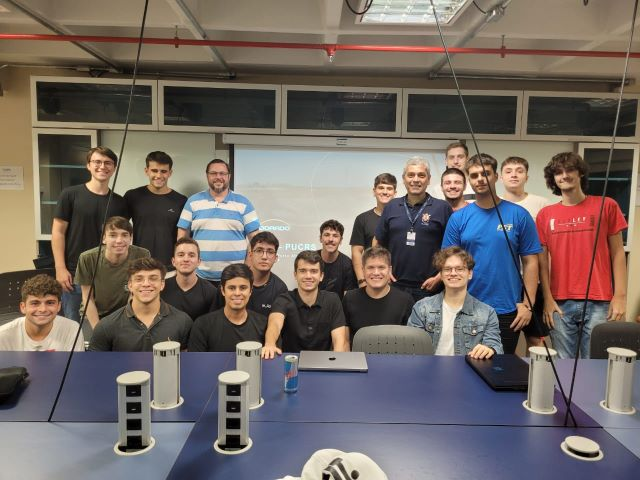
\includegraphics[width=0.8\textwidth]{A.jpg}
    \caption{Time - AGES II}
    \label{fig:exemplo}
\end{figure}

